\section{\Large PROBLEM SET 1}
\subsection{PROBLEM 1}
\textit{Select some key ADCS characteristics of your mission, including orbit (e.g., LEO, MEO, GEO, HEO, Interplanetary), target attitude (e.g., Sun pointing, Inertial pointing, Earth pointing, Resident Space Object pointing), attitude state representation (e.g., Euler angles, Gibbs vector, Quaternions Direction Cosine Matrix, Euler Axis/Angle), sensors suite (Gyros, Magnetometers, Star Trackers, Earth Sensor, Sun Sensor), actuator suite (Thrusters, Magnetorquers, Reaction Wheels, Momentum Wheel, Gravity Gradient).}

The ultimate goal of the project is to work on a satellite using modern observational technologies designed to gather key environmental data on Earth. The satellite will need pointing capabilities that are controlled by the ADCS system.

\subsection{PROBLEM 2}
\textit{Conduct survey of satellites which have characteristics similar to selected project. Use internet, publications, and books as resources.}

Space agencies such as NASA have had a vested interest in being able to gather satellite images and data from Earth for decades now. Because of this, many satellites have been designed to do what we aim to do.

For example, Soil Moisture Active Passive (SMAP) is a NASA satellite launched in 2015 that utilizes L-band synthetic aperture radar (SAR) technology to measure soil moisture from LEO. This data has applications in climate change research climate change research applications (such as updating climate models) and some day-to-day activities (such as improving weather forecasts). SMAP was unique in the sense that it had a large deployable reflector that was attached to a boom \cite{SMAP}. In addition, the companies EOSSAR and Capella Space are developing satellites that use SAR technology in the X-band and S-band regimes for applications ranging from agriculture to mining \cite{EOSSAR, Capella}. Additionally, agencies have been partnering up to create SAR satellites. The most notable example is NASA and ISRO partnering to work on NASA-ISRO Synthetic Aperture Radar (NISAR), which is a satellite that captures data in the L-band and S-band SAR frequencies \cite{NisarMission}. Overall, the unique capabilities of NISAR over the other satellites and the availability of data for it made NISAR the prime candidate for this project.

\subsection{PROBLEM 3}
\textit{Select preferred existing satellite and payload for project. Similarity is helpful, but not strictly required.}

This project will be based on the NISAR satellite.

[IMAGE OF NISAR]

\subsection{PROBLEM 4}
\textit{Collect basic information on mission, requirements, ADCS sensors and actuators, mechanical layout, mass, mass distribution, and inertia properties.}

NISAR is a joint earth-observation satellite missions between NASA and ISRO. It is the first satellite to use two different Synthetic Aperture Radar (SAR) technologies in both the L-band and S-band. Both frequencies can penetrate clouds, but the L-band can penetrate thicker vegetation that the S-band cannot. Meaning, NISAR has the unique ability to be used in far more applications than previous SAR satellites, ranging from disaster response to agriculture cases \cite{NisarApps}.

As shown in \textbf{Figure 1}, NISAR's satellite consists of a 1.9 m x 1.8 m x 1.2 m spacecraft bus cuboid with a 1.2 m wide octagonal Radar Instrument Structure (RIS). The satellite is powered by a 23 m$^2$ solar panel array split on the left and right side of the satellite. Additionally, a 12 m diameter radar antenna is held up by a 9 m long boom with a 7" x 7" cross-section area \cite{NisarMission}.

The table below contains mass properties of the satellite. Unfortunately, mass distribution and inertia properties of NISAR are not publicly available, so they were omitted from the report. However, they are estimated in the next section.

\begin{table}[]
\begin{tabular}{|l|l|}
\hline
\textbf{Component}               & \textbf{Mass (kg)} \\ \hline
Radar Instrument Structure (RIS) & 1375.9             \\ \hline
Spacecraft Bus                   & 964.1              \\ \hline
Radar Antenna Boom (RAB)         & 192                \\ \hline
Radar Antenna Reflector (RAR)    & 100                \\ \hline
Solar Array (total)              & 46                 \\ \hline
Total                            & 2678               \\ \hline
\end{tabular}
\end{table}

Since NISAR is a larger satellite, it has a pretty complex ADCS system with an array of sensors and actuators. On the sensor side, it has a mixture of star sensors; sun sensors; GPS; and 3 gyroscopes used for roll, pitch, and yaw. For actuators, NISAR has four 50 N$\cdot$m reaction wheels mounted tetrahedral, three 565 and 350 A$\cdot$m$^2$ magnetorquers, and fourteen thrusters (ten canted 11 N thrusters, one central 11 N thruster, and four 1 N thrusters for roll) \cite{NisarMission}.



\begin{figure}[H]
\centering
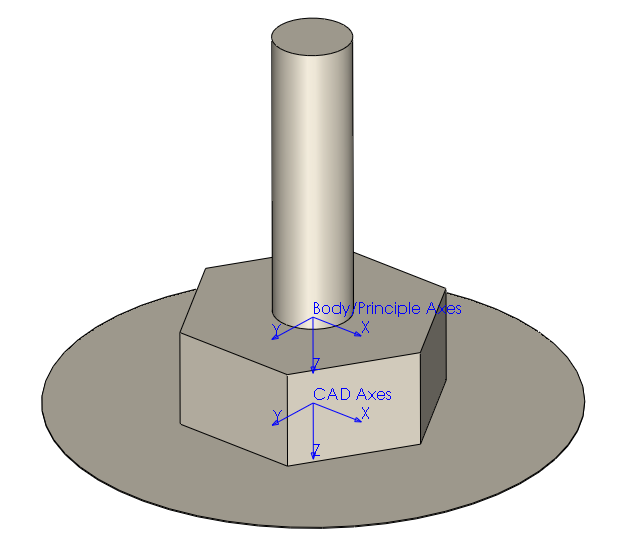
\includegraphics[scale=0.7]{Images/WMAP_CAD4.PNG}
\caption{A 3D model of the simplified satellite geometry. The body and principal axes are labeled and located at the spacecraft center of mass.}
\label{CAD model with frames}
\end{figure}


\begin{equation}
\vec{M} = \vec{I} \cdot \vec{\dot{\omega}}\ + \vec{\omega} \times \vec{I} \cdot \vec{\omega} \\ 
\end{equation}   



\begin{eqnarray}
M_x = I_{xx} \dot{\omega_x} + (I_{zz} - I_{yy})\omega_y \omega_z \nonumber \\
M_y = I_{yy} \dot{\omega_y} + (I_{xx} - I_{zz})\omega_z \omega_x \\
M_z = I_{zz} \dot{\omega_z} + (I_{yy} - I_{xx})\omega_x \omega_y \nonumber
\end{eqnarray}

\begin{equation}
I_{B} =
\begin{bmatrix} 
I_{xx} & I_{xy} & I_{xz} \\
I_{yx} & I_{yy} & I_{yz} \\ 
I_{zx} & I_{zy} & I_{zz} \\
\end{bmatrix}
=
\begin{bmatrix}
1005.5 & 0 & 0 \\
0 & 1005.5 & 0 \\ 
0 & 0 & 543.7
\end{bmatrix}
[kg/m^2].
\end{equation}

\begin{lstlisting}
function L_loc = LagrangePoints(mu)
%For a given value of mu, this function computes the location
%of all five Lagrange points for the circular restricted three
%body problem.

%Compute the location of the libration points
    l = 1 - mu;

    L_loc = zeros(5,3);

    %L1
    p_L1 = [1, 2*(mu - l), l^2 - 4*l*mu + mu^2, 2*mu*l*(l - mu) + mu - l,...
        mu^2*l^2 + 2*(l^2 + mu^2), mu^3 - l^3];
    L1roots = roots(p_L1);
    L1 = 0;
    for i = 1:5
        if (L1roots(i) > -mu) & (L1roots(i) < l)
         L1 = L1roots(i);
        end
    end
    L_loc(1,1) = L1;

    %L2
    %L3
    %L4
    %L5
end
\end{lstlisting}
